\documentclass[10pt,draftclsnofoot,onecolumn]{IEEEtran}

\usepackage{setspace}
\usepackage{caption}

% *** GRAPHICS RELATED PACKAGES ***
\ifCLASSINFOpdf
  \usepackage[pdftex]{graphicx}
  % declare the path(s) where your graphic files are
  \graphicspath{images/}
  % and their extensions so you won't have to specify these with
  % every instance of \includegraphics
  \DeclareGraphicsExtensions{.pdf,.jpeg,.png}
\else
  % or other class option (dvipsone, dvipdf, if not using dvips). graphicx
  % will default to the driver specified in the system graphics.cfg if no
  % driver is specified.
  % \usepackage[dvips]{graphicx}
  % declare the path(s) where your graphic files are
  % \graphicspath{{../eps/}}
  % and their extensions so you won't have to specify these with
  % every instance of \includegraphics
  % \{.eps}
\fi

% correct bad hyphenation here
\hyphenation{op-tical net-works semi-conduc-tor}

\begin{document}
\pagenumbering{gobble}
\singlespacing
\title{Spatial Visualization\\ of Biodiversity}

\author{Ty~Skelton,
        Jasper~LaFortune,
        and~Alec~Shields}% <-this % stops a space


% The paper headers
\markboth{CS 461}%
{Winter 2016}

% make the title area
\maketitle

% As a general rule, do not put math, special symbols or citations
% in the abstract or keywords.
\begin{abstract} % @TODO: JASPER
The Department of Integrative Biology at Oregon State has collected a large sample of biodiversity data from various sites in the Southwest United States.
Handling this data in its raw form requires certain technical knowledge of databases, as well as a bit of patience.
This presents a problem for biodiversity researchers and Department of Defense land managers, who need to be able to understand and make decisions about this data easily.
Our team will address this problem by creating a web interface for spatially visualizing this data.
We will enable users to easily display useful graphs and maps about areas and species of interest, putting the information they care about most at their fingertips.

The Department of Defense made an investment in collecting all these samples so that it could better manage its land.
However, extracting meaning from that information is challenging for land managers and researchers alike.
A good solution to this problem would allow users to easily access the information that is important to them.
Our solution will provide an interface that allows users to select information of interest and see it in map and graph form.
Passerby at Expo will be invited to interact with our system and discover meaningful biodiversity patterns for themselves.
Oregon State biodiversity researchers will provide feedback on how well our product meets their needs.

\end{abstract}
\IEEEpeerreviewmaketitle

\newpage
\pagenumbering{arabic}

\section{Project Purposes and Goals} % @TODO: JASPER
This project aims to aid researchers and land managers in drawing meaningful conclusions from a large set of insect biodiversity data.
The Department of Defense funded researchers to collect insect samples from many sites across the American Southwest over five years.
The resulting dataset is too cumbersome to make sense of in raw form, especially for land managers with little formal knowledge of database operations.
Our goal is to create a visualization system that allows these parties to select information of interest, display it on a map, and show useful graphs about it.

These requirements led us to a design comprised of three views.
The Filter View allows users to select which data will be displayed by date, season, species, or location.
The Map View shows the locations of the selected samples.
The Graph View shows graphs of the data selected in the Filter View broken down by location, taxa, and time.


\section{Progress}

\subsection{Base Website Setup} % @NOTE: TY - Base Website Setup
When we were doing our technology review in preparation for writing our design document, we decided on using Django for our web framework, Apache for our web server, Git for our version control system, MySQL for our database, Bootstrap for our front end framework, and c3/arcGIS for our graphing/map views.
We’ve since organized and set up our back-end web framework correctly for our web app.
Since Django ships its beginning web structure in a very minimalistic state, (i.e. their templates, views, and models all in just one file with no app structure) We had to modularize those components into their own directories and files.
It wasn’t a long and arduous process, but it did take a bit of time learning how to go about doing that since we were all new to using Django.

Our web server configuration for development is fairly minimal at the moment.
We are still development, which means we’re making all of our features on our local machines.
However, we are now beginning the process of deployment and have gone through the proper channels for gaining access to a remote server that we will put our web tool on.
Apache does not require much set up to deploy your projects to localhost.
The only real challenge with getting Apache up and running was installing one dependency called MOD-WSGI which is required for Apache to serve Django content to the web, even on localhost.

Tracking our progress in development has been a breeze with Github.
We use the branching feature for each of us to introduce new features to our project.
Since each of us is in charge of one view (functionality) branching that is very easy and we still use it for making core changes to the framework.
We also track new features and issues with Git’s issue tracker and assign them all to milestones so we can properly prioritize changes by whether or not they’re in the coming release.

We all have some amount of experience interacting with MySQL, whether it be from our database class we took in pre-pro school or in the work force. That made converting our sponsor’s access database to MySQL much easier than it could’ve been, but it still was very challenging.
We have our system tied to the database perfectly and we are rendering data from it on our web page in different sections for a proof of concept.

Our front end framework we chose to implement was Bootstrap.
Bootstrap is a very well defined CSS/HTML framework and has seen use all kinds of applications, whatever the scale.

\subsection{Main Layout} % @NOTE: TY - Main Layout
As dictated in the design document, the main layout of the index page of our app is split into three sections.
Each section has been individually developed by each member of the team.
The top right view has an interactive map in a container.
In the top left there is a panel for filtering the data that is supplied to the other two views.
It has drop downs and date filters for better narrowing a field of data to fit what the user is looking for.
Finally, the index’s bottom container has a side-scrolling graph view that provides useful metrics on what the data consists of.
Each contained view has its own template that is embedded in a primary main template in an effort to keep the main template clean and organized.

\begin{figure}[h]
\centering
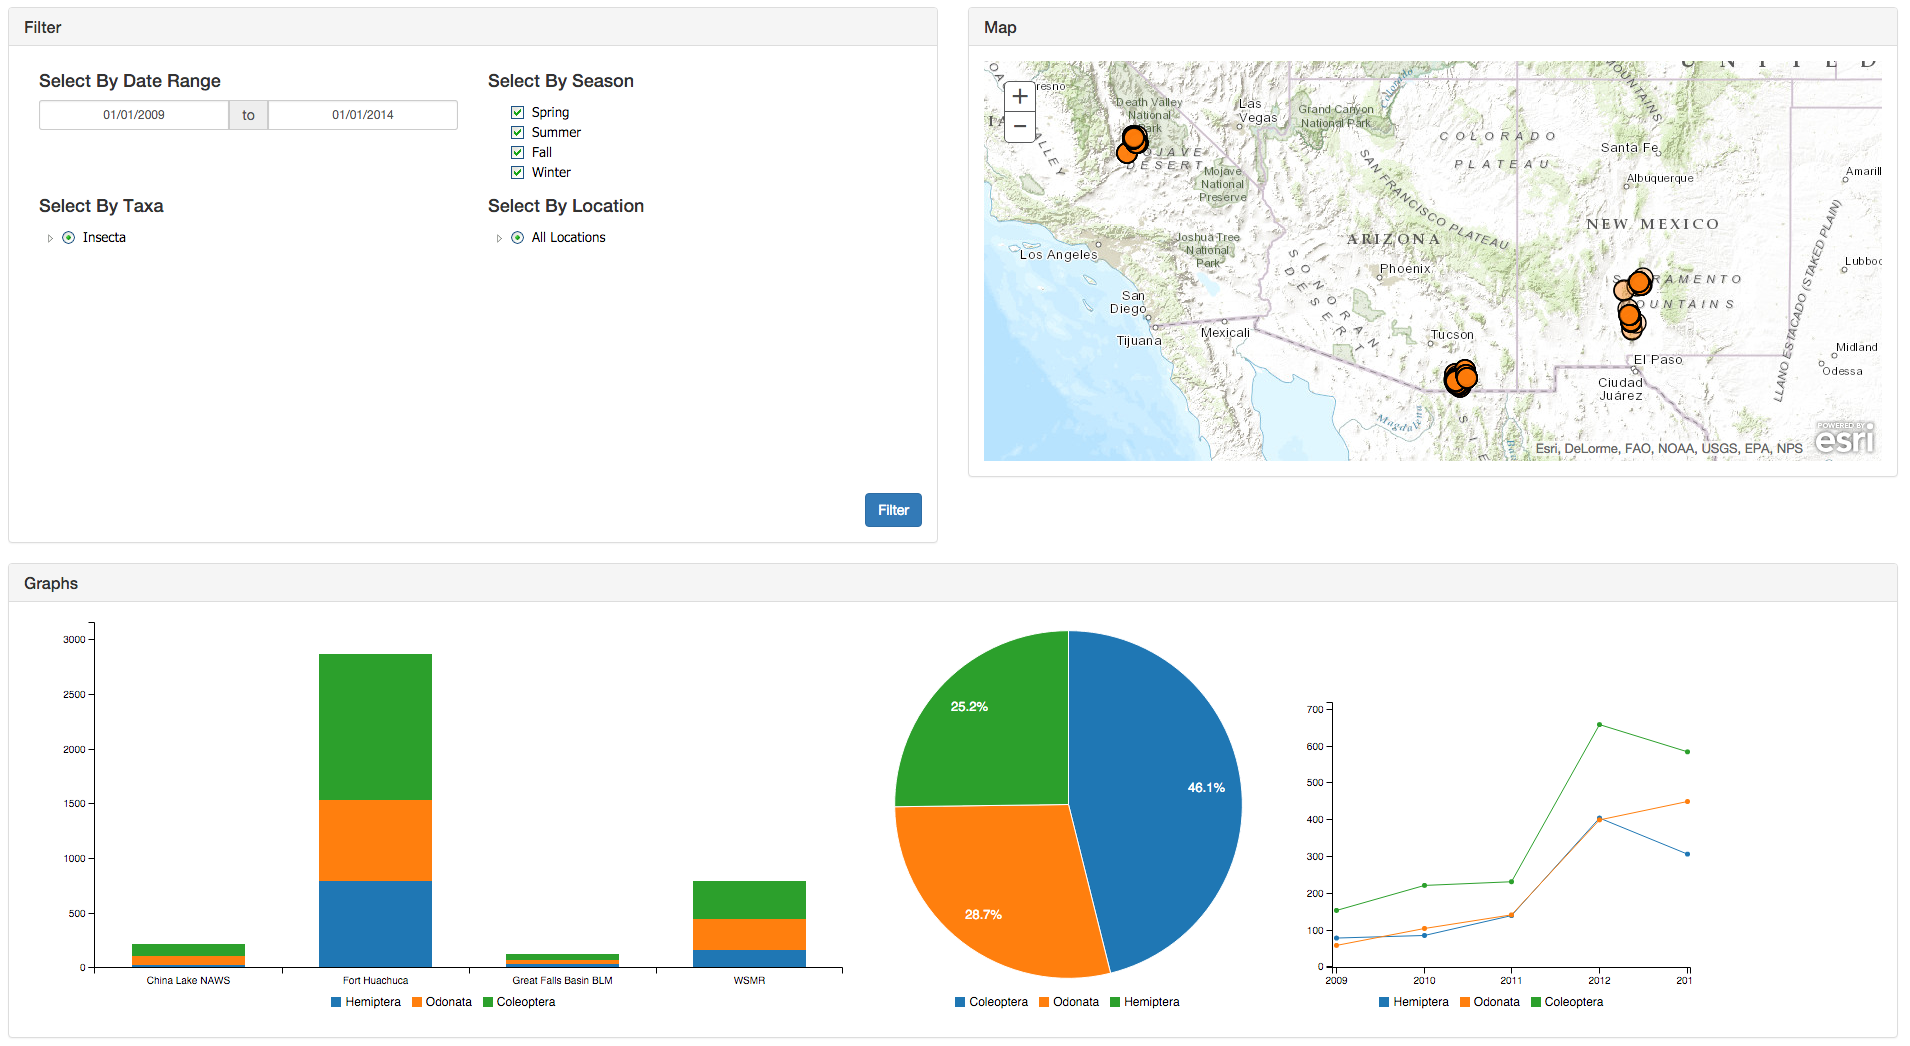
\includegraphics[width=0.75\textwidth]{images/main_layout.png}
\captionsetup{justification=centering}
\caption{
  Overall site layout view.
  upper left: filter view, upper right: map view, bottom: graph view.
}
\label{fig:layout}
\end{figure}

The main challenge with developing our single page web-app was providing data to the various tools we’re making use of in our different containers.
We have written models that map objects to database entries and allow us to provide serialized data to our templates.

\subsection{Filter View} % @TODO: JASPER

The Filter View allows users to select information of interest by date, season, biological taxonomy, or site.
Selections made in the Filter View affect what is shown in the Map and Graph Views.
When the Filter View first loads, the user sees the pane shown in Figure~\ref{fig:overall_filter}.
By default, all data are selected.
The Date Range Filter begins populated with dates that capture the full range of data collection.
The Season Filter begins with all four seasons selected.
The Taxa Filter and the Site Filter begin fully collapsed, with the highest level selected.

\begin{figure}[h]
\centering
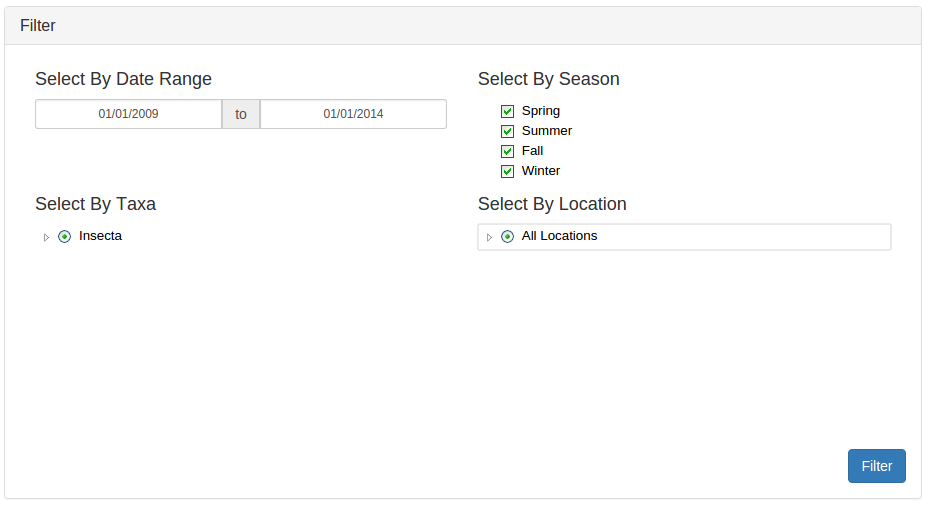
\includegraphics[width=0.75\textwidth]{images/overall_filter.png}
\captionsetup{justification=centering}
\caption{
  The Filter view contains four tiled filters, Date, Season, Taxa, and Location.
  By default, all data are selected and all children collapsed.
}
\label{fig:overall_filter}
\end{figure}

When the user makes selections in the Filter View, the Filter button changes color, as demonstrated in Figure~\ref{fig:date_filter}.
Clicking on the Filter button applies the selections made in the Filter View to the other two views.
Selections made in the Filter View persist on submission, so that the user can make selections serially.

The Date Filter allows users to view data from between a range of dates.
Clicking on either date field opens up a date range picker, shown in Figure~\ref{fig:date_filter}.
Users can also type in the date manually.
This causes the Graph View to only graph data collected between these two dates.
The Season Filter allows users to view data collected during certain seasons across all years.

\begin{figure}[h]
\centering
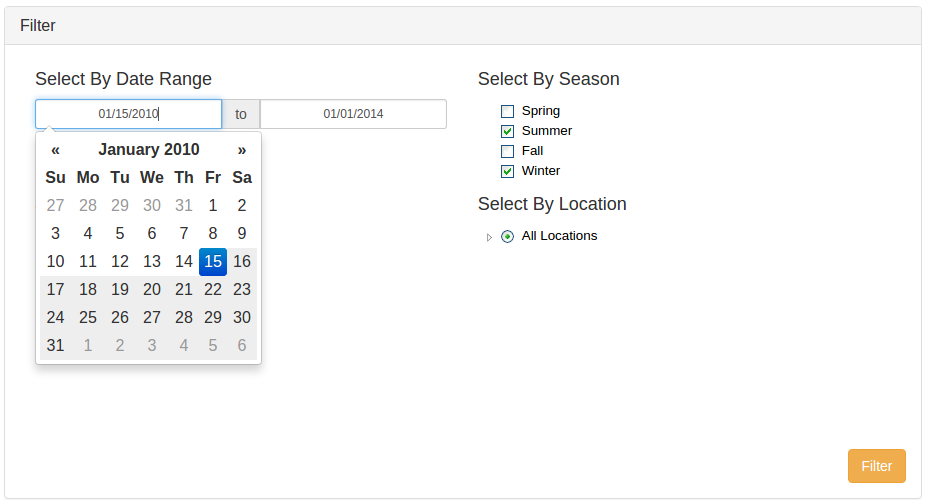
\includegraphics[width=0.75\textwidth]{images/date_filter.png}
\label{fig:date_filter}
\captionsetup{justification=centering}
\caption{
  When selections are made in the Filter View, the Filter Button changes color to indicate that submission is necessary.
  The Date Filter includes a date range picker.
}
\end{figure}

The Taxa Filter, shown in Figure~\ref{fig:taxa_filter}, allows users to select orders, families, genus, and species of interest hierarchically.
Users can select a radio button at any level in the hierarchy.
Selecting a parent node in the Taxa Filter supplies all the data from its children and none of the data from its siblings to the Graph View.
The Site Filter, shown in Figure~\ref{fig:location_filter}, allows users to select bases, drainages, sites, and samples of interest hierarchically.
Selecting a parent node in the Site Filter supplies all the data from its children and none of the data from its siblings to the Graph and Map Views.
Users can click on the triangle next to each parent to toggle whether its children are collapsed or expanded.
Expanding or collapsing children simply determines whether or not they show on screen, and does not affect selection.

\begin{figure}[h]
\centering
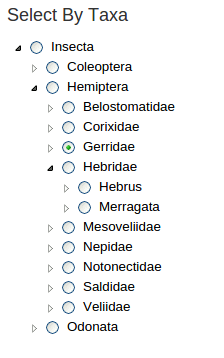
\includegraphics[width=0.25\textwidth]{images/taxa_filter.png}
\captionsetup{justification=centering}
\caption{
  The Taxa Filter allows the user to select an arbitrary level of biological taxonomy and all its children.
  For example, selecting the family Gerridae in the order Hemiptera selects all genuses and species inthe Gerridae family.
  Because the input is a radio button, the user cannot simultaneously select siblings.
}
\label{fig:taxa_filter}
\end{figure}

\begin{figure}[h]
\centering
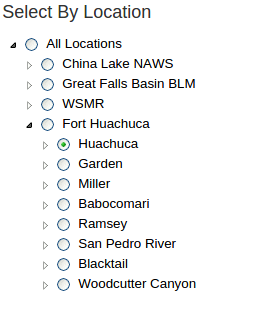
\includegraphics[width=0.25\textwidth]{images/location_filter.png}
\captionsetup{justification=centering}
\caption{
  The Location Filter allows the user to select an arbitrary location and all its children.
  For example, selecting the Huachuca drainage at the Fort Huachuca Base selects all sites in that drainage and all samples in those sites.
  Because the input is a radio button, the user cannot simultaneously select siblings.
}
\label{fig:location_filter}
\end{figure}

Jasper was assigned to developing the Filter View.
The main obstacle he faced was not any of the filters themselves, but rather the learning curve for the development workflow.
His experience using git for collaborative projects was limited, so on multiple occasions he called for help from the others.
His experience with web development was also limited, so tasks such as setting up a server required assistance.

When it came to writing code, the Filter View presented two main challenges.
The first was extracting meaningful information from the data posted by the filters.
To do this, we created a Filter Helper class that populates a dictionary with all the relevant fields for refining queries.
The second major challenge was making filter selections persistent.
To do this, we had to embed code in our html template to populate the fields from the data in the Filter Helper dictionary.
As such, data flows from the input forms in the Filter View, to the Filter Helper dictionary, back to the input forms.

\subsection{Map View} % @TODO: ALEC

\subsection{Graph View} % @NOTE: TY - Graph View
The graph view portion of our web tool is beta-level ready.
We have fully developed charts deployed that render dynamically-loaded data based off of filter input.
Our goal with these graphs for the beta release was to have each one not only pulling in data from the database, but rendering it in the correct way with x-values and labels set to whatever the parameters of interest implied.
While we have three graphs that show exactly what our sponsor requested, we still have a little bit of honing to do in terms of a stretch goal to get very specific graphs to display.
We are able to customize every aspect of them in regards to color, spacing, font, layout, etc.
An example of what the graph-portion looks like is shown in Figure~\ref{fig:graph_view}.
When the page is resized to be smaller, the graph window view will display a horizontal scroll bar so that the user can still see the metrics they’re interested in without having to scrunch them up.

\begin{figure}[h]
\centering
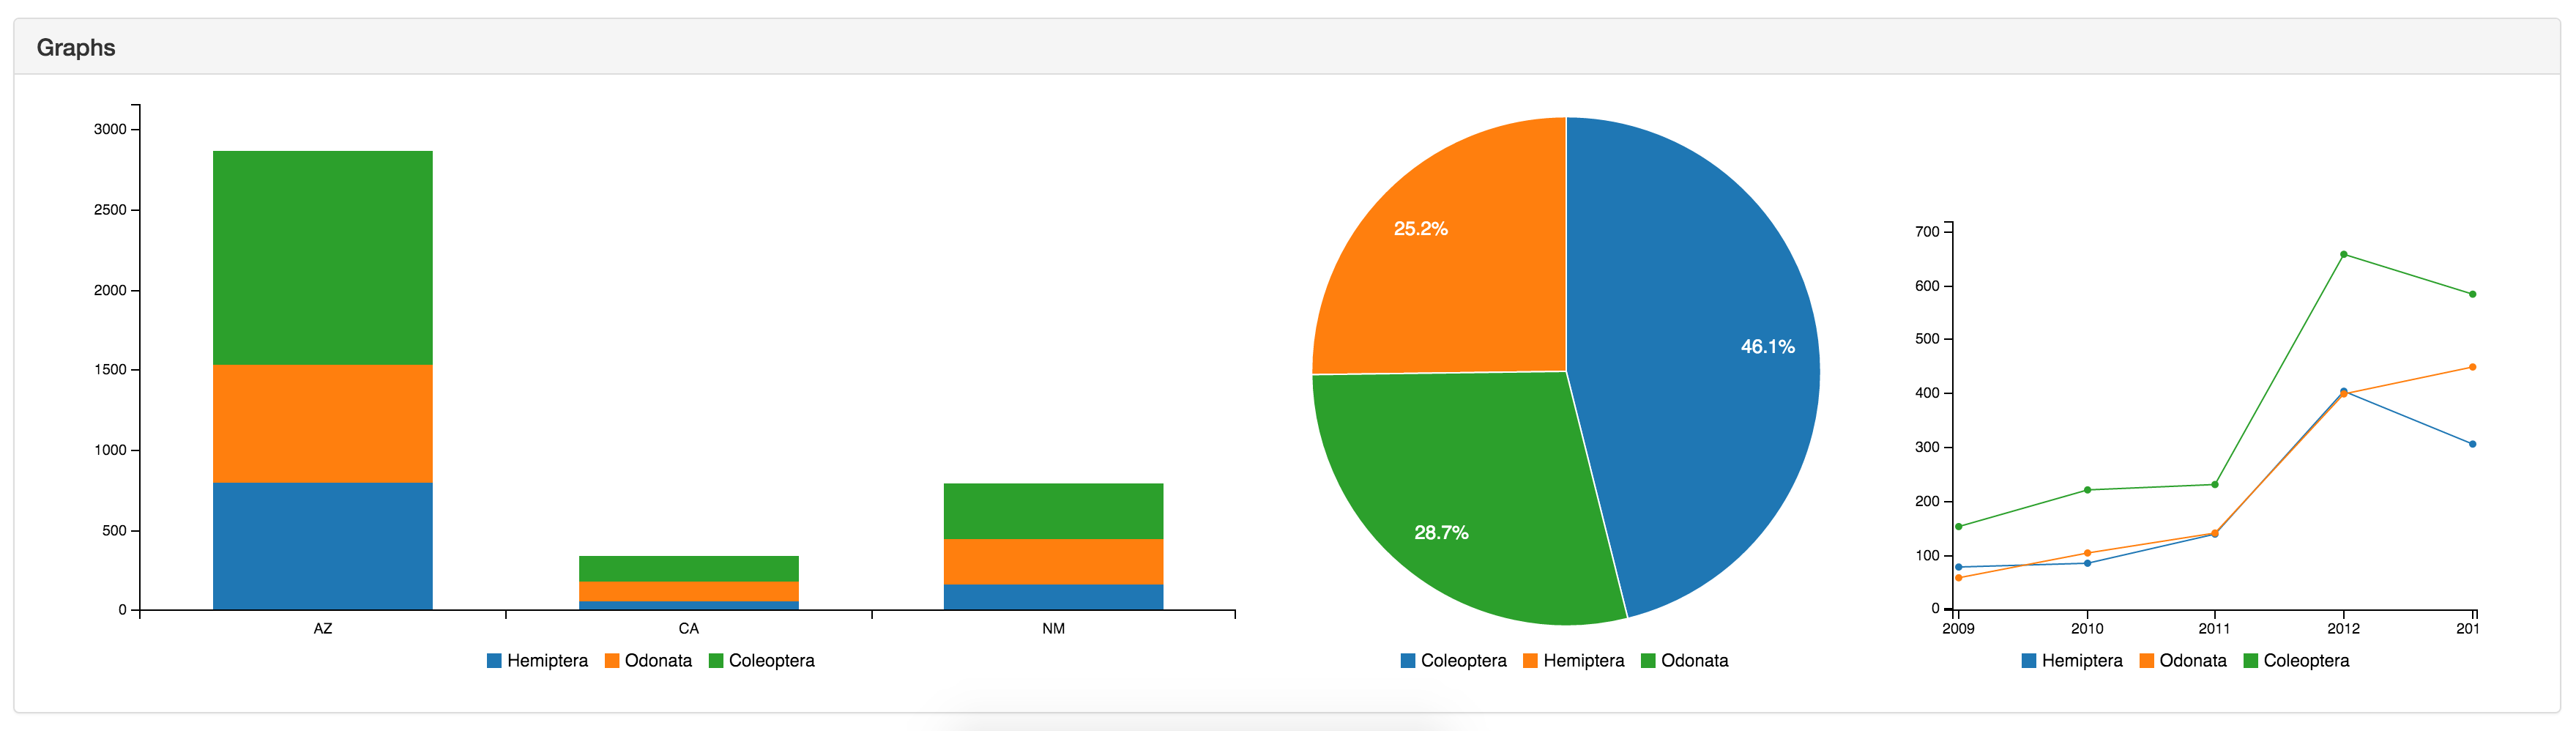
\includegraphics[width=0.75\textwidth]{images/graph_view.jpg}
\captionsetup{justification=centering}
\caption{
  The overall graph view.
  Displays dynamically generated charts on every page load and filter submission.
}
\label{fig:graph_view}
\end{figure}

The three different graphs that we were successfully able to pull data into and render meaningful statistics in were the stacked bar chat, pie chart and line chart.
The stacked bar chart is showing the number of unique taxa within a certain taxonomic level at each location.
The pie chart is showing the distribution of unique taxa overall for all locations within the scope selected by the user.
Finally, the line chart is showing the number of unique taxa observed across all locations over time (years).

After the filter view submits a POST request to the index controller and figures out the parameters of interest (described in the filter section) an object with the necessary information is passed to the graph view.
Since the currency for the graph view is unique taxa observed, all the database queries and data massaging takes place in the subsample model.
After a particular graph retrieves the filter object it passes a generic query and refines it based on what the user is interested in.
Django uses lazy loading, meaning the query object is never processed until the code tries to parse it.
After the model gets the necessary information it has to format the two dimensional array in a very peculiar fashion for our graphing library to handle it (C3.js).
After it's formatted correctly, the model returns the array of arrays to the view, which stores it in the data object that is embedded in the view.
C3.js is loaded in the template as well, so we just embed the data object using Django's templating tools so it's parsed on load after all the dependencies.

\begin{figure}[h]
\centering
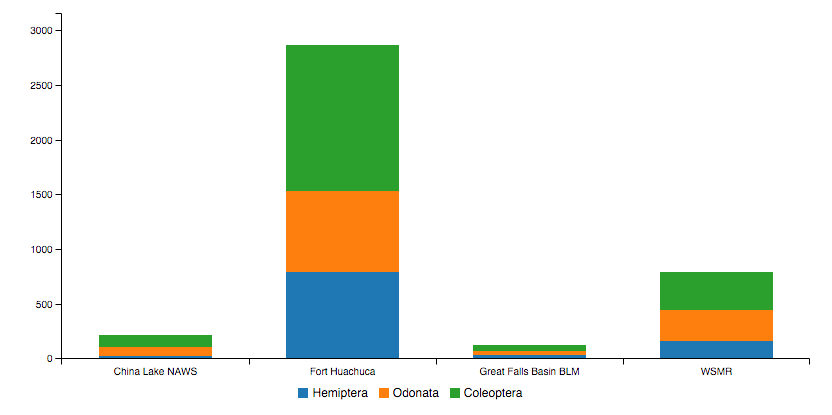
\includegraphics[width=0.70\textwidth]{images/bar_chart.png}
\captionsetup{justification=centering}
\caption{
  Stacked bar chart showing counts of unique taxa observed within a specified taxonomic level across varying locations.
}
\label{fig:bar_chart}
\end{figure}

The graph in Figure~\ref{fig:bar_chart_collapsed} displays a functionality in c3 that is really useful and is one of the primary reasons that we chose c3 as our graphing library for development.
If the user is to click (or touch on a touchpad) the label for a particular dataset within a graph, then the graph will hide that dataset and focus on only the remaining.
This is a very important functionality, because when taking biodiversity readings there could be an under-represented species or genus that only shares a small percentage of the dataset.
There could even be multiple that are dominated by one large collection.
If the user wants to ‘zoom in’ on those particular small readings, they could just hide the dominating dataset by clicking its label.

\begin{figure}[h]
\centering
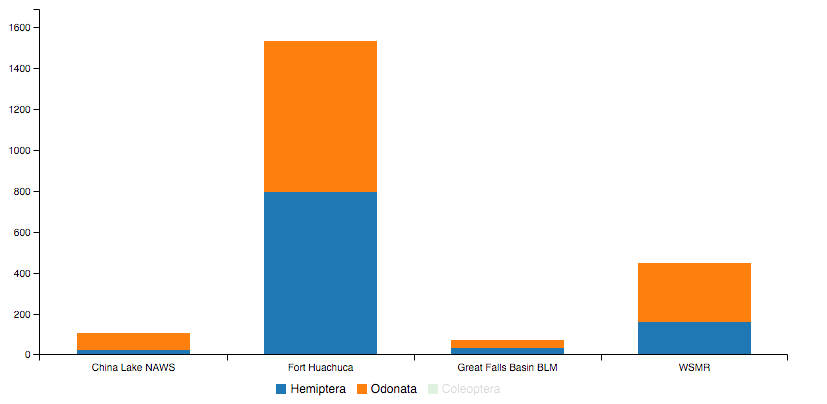
\includegraphics[width=0.70\textwidth]{images/bar_chart_collapsed.png}
\captionsetup{justification=centering}
\caption{
  An example of how the labels can be clicked to hide certain data displayed from view so the user can zero-in on a particular dataset.
}
\label{fig:bar_chart_collapsed}
\end{figure}

During development we encountered some varyingly-sized problems that slowed us down, but we were able to overcome them before beta release.
The ability to supply data and render accurate graphs dynamically was our goal for the graph view come beta release, but it took some hard work to get it to the point it's at.
None of us have used Django in the past and its ORM (object relational mapping) model structure, for constructing and querying objects from the database, was completely foreign to us.
Once we were able to learn how Django does it’s aggregate queries to the database it became a little bit more clear how to perform our queries, but it still proves to be challenging.
Early on after alpha release we were able to get all the static data supplied to the graphs replaced with dynamic data.
The end was in sight, but the ability to render dynamic x-values, labels, and y-values quickly became very difficult and it required a lot of clever problem solving to find a way to piggy-back data filtration logic in our filter helper models.
Once we were able to break through those barriers everything seemed to tone down in difficulty.
As we enter into the production-level phase of development we'll be doing much more polish and refinement than actual feature implementation, which is where we wanted to be.

\subsection{Database and Preparing Data}
% @TODO: ALEC

\end{document}
